\RequirePackage{luatex85}
\documentclass[amsmath]{article}
\usepackage{amsmath}
\usepackage{amssymb}
\usepackage{geometry,contour}
\usepackage{tikz}
\usetikzlibrary{positioning}
\usetikzlibrary{decorations.text}
\usetikzlibrary{decorations.pathmorphing}
\usetikzlibrary{decorations.text}
\usetikzlibrary{decorations.pathmorphing}
\definecolor{darkolivegreen}{rgb}{0.3, 0.5, 0.2}
\geometry{legalpaper, landscape, margin=0.0in}
\paperheight 2.4in
\paperwidth 5.2in


\begin{document}
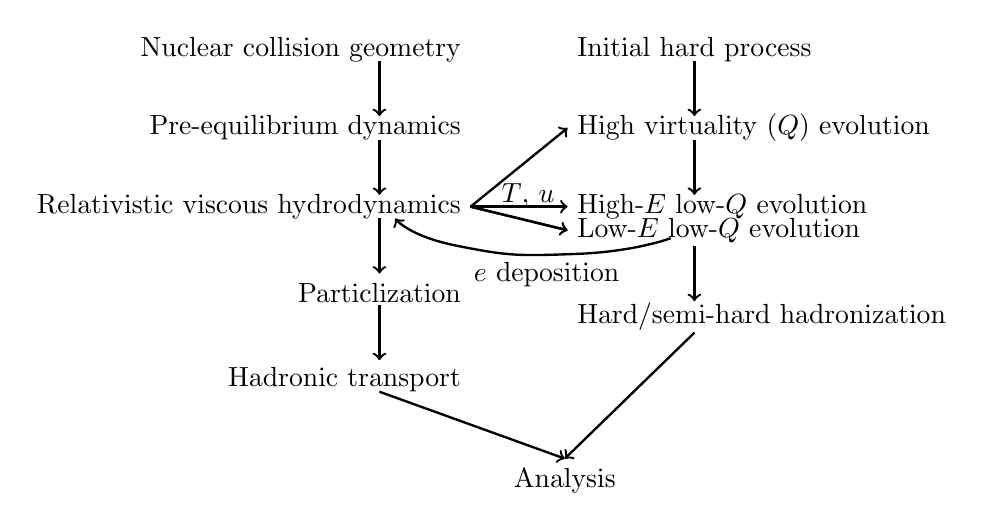
\begin{tikzpicture}
\node(a)[align=right] at (0,0) {Nuclear collision geometry};
\node(A)[align=right] at (5,0) {Initial hard process};

\node(b)[below=of a.east, yshift=0cm, anchor=east]  {Pre-equilibrium dynamics};
\node(B)[below=of A.west, yshift=0cm, anchor=west] {High virtuality ($Q$) evolution};

\node(c)[below=of b.east, yshift=0cm,anchor=east] {Relativistic viscous hydrodynamics};
\node(C)[below=of B.west, yshift=0cm,anchor=west]{High-$E$ low-$Q$ evolution};
\node(C2)[below=of B.west, yshift=-.3cm,anchor=west]{Low-$E$ low-$Q$ evolution};

\node(d)[below=of c.east, yshift=-.1cm,anchor=east]  {Particlization};
\node(e)[below=of d.east, yshift=-.1cm,anchor=east] {Hadronic transport};

\node(D)[below=of C2.west, yshift=-.1cm,anchor=west]  {Hard/semi-hard hadronization};

\node(E)[below=of D.south, xshift=-2.5cm, yshift=-.5cm] {Analysis};

\draw[->, color=black,line width=.3mm] (1,-.15)--(1,-.85);
\draw[->, color=black,line width=.3mm] (1,-1.15)--(1,-1.85);
\draw[->, color=black,line width=.3mm] (1,-2.15)--(1,-2.85);
\draw[->, color=black,line width=.3mm] (1,-3.25)--(1,-3.95);
\draw[->, color=black,line width=.3mm] (1,-4.35)--(E.north);

\draw[->, color=black,line width=.3mm] (5,-.15)--(5,-.85);
\draw[->, color=black,line width=.3mm] (5,-1.15)--(5,-1.85);
\draw[->, color=black,line width=.3mm] (5,-2.5)--(5,-3.2);
\draw[->, color=black,line width=.3mm] (5,-3.6)--(E.north);

\draw[->, color=black,line width=.3mm] (c.east)--(B.west);
\draw[->, color=black,line width=.3mm] (c.east)--(C.west);
\draw[->, color=black,line width=.3mm] (c.east)--(C2.west);

\draw[->, color=black,line width=.3mm] (c.east)--(C2.west);


\path [->, decorate,decoration={text along path,
            text={~~~$T$, $u$}}]
 (2.2, -1.95)--(4.3,-1.95);
 
 \draw [->, color=black,line width=.3mm] plot [smooth, tension=1] coordinates { (4.7, -2.4) (3.5,-2.6)(2, -2.5)(1.2, -2.15)};
\path [->, decorate,decoration={text along path,
            text={$e$ deposition}}]
 (2.2, -2.95)--(4.5,-2.95); 
\end{tikzpicture}

\newpage  
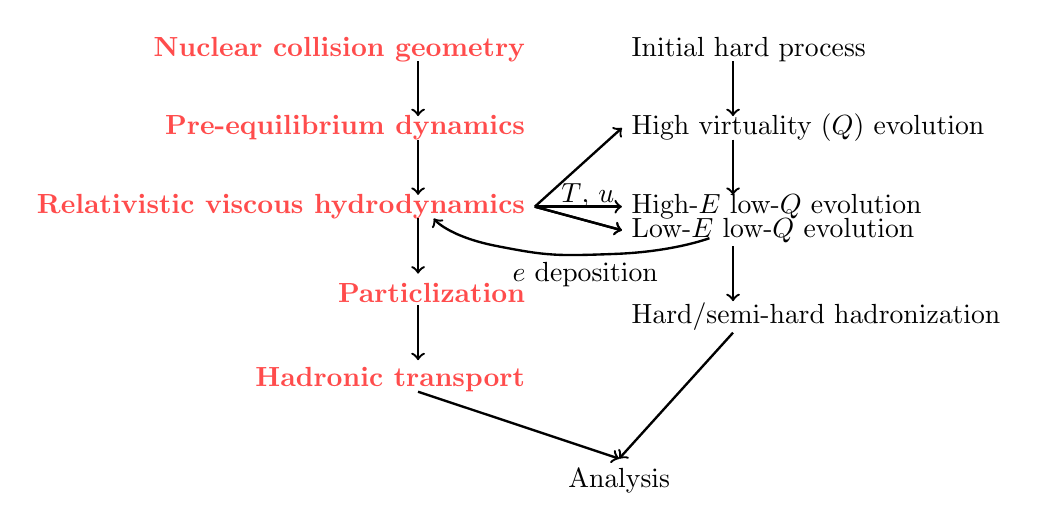
\begin{tikzpicture}
\node(a)[align=right] at (0,0) {\bf \color{red!70}Nuclear collision geometry};
\node(A)[align=right] at (5.2,0) {Initial hard process};

\node(b)[below=of a.east, yshift=0cm, anchor=east]  {\bf \color{red!70}Pre-equilibrium dynamics};
\node(B)[below=of A.west, yshift=0cm, anchor=west] {High virtuality ($Q$) evolution};

\node(c)[below=of b.east, yshift=0cm,anchor=east] {\bf \color{red!70}Relativistic viscous hydrodynamics};
\node(C)[below=of B.west, yshift=0cm,anchor=west]{High-$E$ low-$Q$ evolution};
\node(C2)[below=of B.west, yshift=-.3cm,anchor=west]{Low-$E$ low-$Q$ evolution};

\node(d)[below=of c.east, yshift=-.1cm,anchor=east]  {\bf \color{red!70}Particlization};
\node(e)[below=of d.east, yshift=-.1cm,anchor=east] {\bf \color{red!70}Hadronic transport};

\node(D)[below=of C2.west, yshift=-.1cm,anchor=west]  {Hard/semi-hard hadronization};

\node(E)[below=of D.south, xshift=-2.5cm, yshift=-.5cm] {Analysis};

\draw[->, color=black,line width=.3mm] (1,-.15)--(1,-.85);
\draw[->, color=black,line width=.3mm] (1,-1.15)--(1,-1.85);
\draw[->, color=black,line width=.3mm] (1,-2.15)--(1,-2.85);
\draw[->, color=black,line width=.3mm] (1,-3.25)--(1,-3.95);
\draw[->, color=black,line width=.3mm] (1,-4.35)--(E.north);

\draw[->, color=black,line width=.3mm] (5,-.15)--(5,-.85);
\draw[->, color=black,line width=.3mm] (5,-1.15)--(5,-1.85);
\draw[->, color=black,line width=.3mm] (5,-2.5)--(5,-3.2);
\draw[->, color=black,line width=.3mm] (5,-3.6)--(E.north);

\draw[->, color=black,line width=.3mm] (c.east)--(B.west);
\draw[->, color=black,line width=.3mm] (c.east)--(C.west);
\draw[->, color=black,line width=.3mm] (c.east)--(C2.west);

\draw[->, color=black,line width=.3mm] (c.east)--(C2.west);


\path [->, decorate,decoration={text along path,
            text={~~~$T$, $u$}}]
 (2.47, -1.95)--(4.3,-1.95);
 
 \draw [->, color=black,line width=.3mm] plot [smooth, tension=1] coordinates { (4.7, -2.4) (3.5,-2.6)(2, -2.5)(1.2, -2.15)};
\path [->, decorate,decoration={text along path,
            text={$e$ deposition}}]
 (2.2, -2.95)--(4.5,-2.95); 
\end{tikzpicture}

\end{document}

